\section{Results}
\label{sec:results}

Through this section we discuss the experimental tested along with the valuation strategy carried out. 

The main purpose of our test is to understand how many tags for each service are correctly addressed. In order to achieve this, we have distributed GHio-Ca to some testers and asked to deselect tags that doesn't concern photos that they have taken. Finally, they have to send the result to us.

Our approch was to make as simple as possible for the tester to contribute: we (i) made a video tutorial in which we have shown what they had to do, (ii) wrote a mini-wiki where the experiment was explained, (iii) modified the application. 

According to our planification, to each testing member was asked to take 5 photos.

\subsection{Tester version vs Normal one}
We needed to do three main edits to the normal version to be able to carry on the experiment. The first one is about the way we retrieved results from services. In the normal app version the tags are merged together, instead in the test version we did not.
Abusing the API calls from users was our concern, and to solve this we put a limit on the maximum number of pictures that a tester can take.
Last but not least is how the results are shared. With the test version we only allowed users to share the content with e-mail applications, sending tags and photos to our email address.

% o7

\subsection{Graphical analysis}

At the end of the testing phase, we collected all the e-mails recieved, we counted it and, thanks to \texttt{R}, we built serval graphical rappresentations that we will explain.

\begin{figure}[H]
\centering
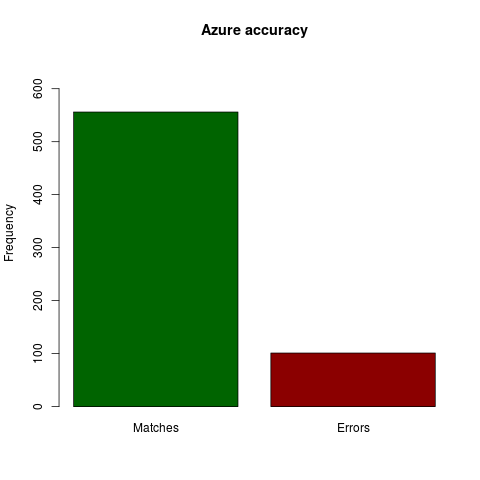
\includegraphics[scale=0.4]{AzureGraph}
\caption{Graphical rapresentation of Azure tags}
\label{testgraphsazure}
\end{figure}

As we can see in Figure~ \ref{testgraphsazure}, Azure behaviour is pretty good, with 85\% circa of correct tags. This is the best result we are able to obtain.

\begin{figure}[H]
\centering
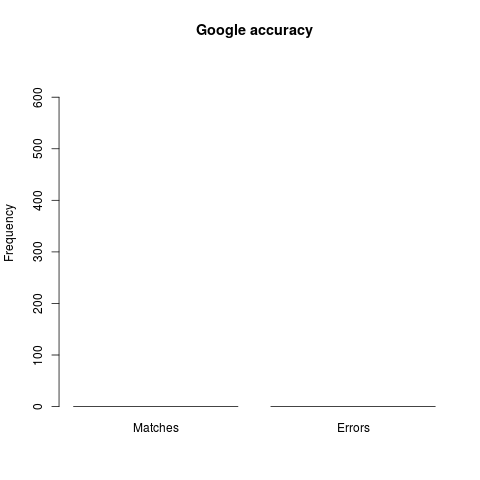
\includegraphics[scale=0.4]{GoogleGraph}
\caption{Graphical rapresentation of Google tags}
\label{testgraphgoogle}
\end{figure}

As we can see, using Google Imae search, we obtained the worst performance among the services we used. Rarely we had tags from this service, with 32 tags only 10 were correct, with a 31\% of correct tags. As a matter of fact, Google Image search was not designed to provide tags from/to user images, thus we did not expect good results from this service.

\begin{figure}[H]
\centering
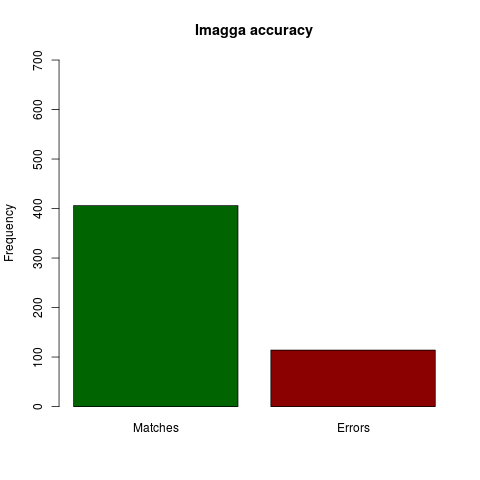
\includegraphics[scale=0.4]{ImaggaGraph}
\caption{Graphical rapresentation of Imagga tags}
\label{testgraphimagga}
\end{figure}

Imagga is an minor service that we discorvered searching online. This provider give us 78\% of correct tags. Is important to keep in mind that most of the bad tags were filtered by our application before getting diplayed to the user. We displayed tags with more than 0.7 of confidence.

\begin{figure}[H]
\centering
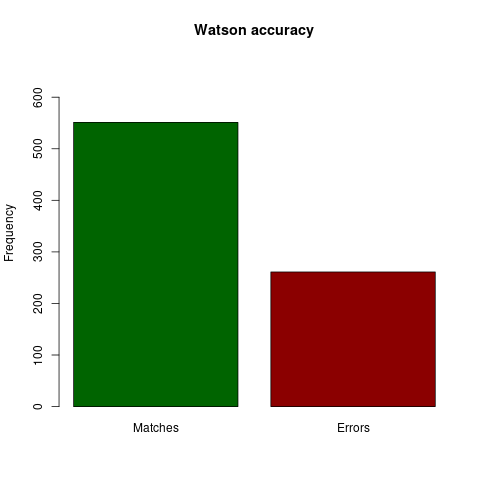
\includegraphics[scale=0.4]{WatsonGraph}
\caption{Graphical rapresentation of Watson tags}
\label{testgraphwatson}
\end{figure}

Watson is an IBM service for image recognition. From the results we observed that the service provided a lot of tags, but a good chunk were wrong, with only 68\% of correct one.

\begin{figure}[H]
\centering
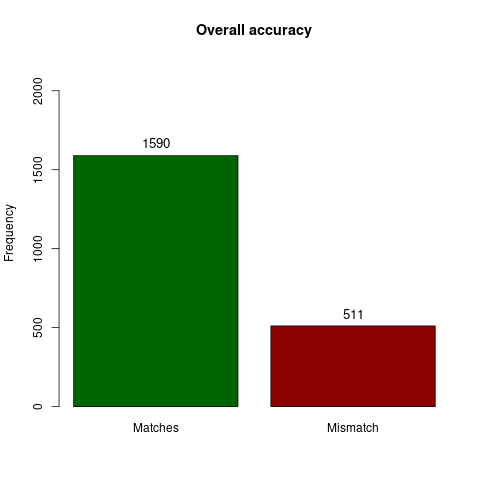
\includegraphics[scale=0.4]{OverallGraph}
\caption{Graphical rapresentation of Watson tags}
\label{testgraphoverall}
\end{figure}

In Figure~ \ref{testgraphoverall} we can see the overall rapresentation, with a percentage of 75\% of correct tags, that we consider it to be a good result.

\subsection{Character recognition}

\begin{figure}[H]
\centering
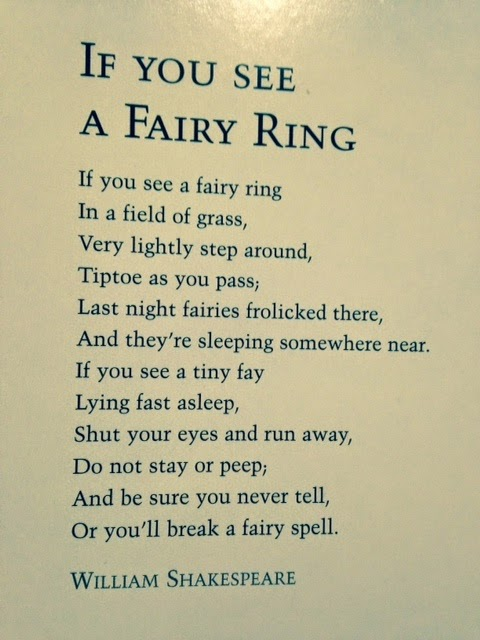
\includegraphics[scale=0.4]{ocr}
\caption{Example of photo with text}
\label{testOCR}
\end{figure}

Execution of OCR on the image~ \ref{testOCR} gives the following result:
\begin{lstlisting}
IF YOU SEE
A FAIRY RING
if you see a fairy ring
in a field of grass,
very lightly step around,
tiptoe as you pass;
last night fairies frolicked there,
and they're sleeping somewhere near.
if you see a tiny fay
lying fast asleep,
shut your eyes and run away,
do not stay or peep;
and be sure you never tell,
or you'll break a fairy spell.
WILLIAM SHAKESPEARE
\end{lstlisting}

In this case we obtain a perfect match. However, with different resolutions and languages, the results are not so good. Unfortunately, we were not able to gain data to build a good evaluation set.